% CSE 655 Term Project - Technical report (draft v0.1, 2026-11-11)
% Numbers come from results/summary.md (row numbers in comments: [S#]).
% Lines marked TODO must be checked or filled before submission.
\documentclass[11pt,a4paper]{article}
\usepackage[margin=2.2cm]{geometry}
\usepackage[T1]{fontenc}
\usepackage{lmodern}
\usepackage{graphicx}
\usepackage{booktabs}
\usepackage{amsmath}
\usepackage{caption}
\usepackage{subcaption}
\usepackage{xcolor}
\usepackage[hidelinks]{hyperref}
\captionsetup{font=small,labelfont=bf}
\graphicspath{{../results/figures/}{../results/visual_check/}}
\newcommand{\kn}{KirazNet}
\newcommand{\todo}[1]{\textcolor{red}{[TODO: #1]}}
\setlength{\parskip}{3pt}

\title{\textbf{Green CNNs for Image Regression:\\Counting Synthetic Cells with the Smallest Carbon Footprint}\\[4pt]
\large CSE 655 Deep Learning --- Term Project}
\author{Halit Batuhan Aslan \quad (220104004003)\\Gebze Technical University}
\date{November 2026}

\begin{document}
\maketitle

\begin{abstract}
We predict the number of cells in synthetic fluorescence microscopy images (BBBC005) and compare a
small CNN designed from scratch, \kn{} (60{,}465 parameters, 37.2\,M MACs per image), with
ImageNet-pretrained MobileNetV3-Small and ResNet-18, a mean predictor and a two-parameter
brightness regression. Every run of the project, including searches, diagnostics and failed runs,
was logged and measured with CodeCarbon (except two untracked checks of a few seconds); the whole project used 32.6\,Wh (15.1\,g CO$_2$eq). On the held-out
test scenes \kn{} reaches an MAE of 1.57 cells with the lowest training footprint of the CNNs
(0.20\,g CO$_2$eq), but it misses the course's acceptance threshold
($1.15\times$ the best standard model, 1.44 cells). Post-hoc validation diagnostics trace the failure
to the choice of a checkpoint on a noisy validation curve, which left a systematic offset of about
+0.8 cells. The strongest result is that the brightness baseline (MAE 1.14) is as accurate as every
CNN at 60--400 times lower inference energy: for this task, the greenest model is not a deep one.
\end{abstract}

% =====================================================================
\section{Problem and dataset}

\textbf{Task.} Given a greyscale microscopy image, predict the number of cells it contains (a
real-valued regression target). Metrics are MAE (primary), RMSE and $R^2$, all in cells.

\textbf{Dataset.} BBBC005 v1 from the Broad Bioimage Benchmark Collection~\cite{ljosa2012}: 19{,}200
8-bit TIF images ($696\times520$) simulated with SIMCEP~\cite{lehmussola2007}. The page releases the
images and ground truth under a CC0 waiver. The count is encoded in the file name. Our inventory
showed that the files are \emph{not} 19{,}200 independent samples: they are 600 simulated scenes
(24 counts from 1 to 100 $\times$ 25 samples), each rendered at 16 blur levels and in 2 stains.
Same-scene images at F1 and F48 correlate at $r\approx0.89$, different scenes at $r\approx0$.

\textbf{Subset (chosen by pre-registered rules, Appendix~A).}
\begin{itemize}\setlength\itemsep{0pt}
\item \emph{Stain.} The documentation says stain 2 is nuclei. Our pixel test (Otsu objects on C1 F1)
showed the opposite: the w1 object lies fully inside the w2 object (containment 1.00) and is
3--4$\times$ smaller (Fig.~\ref{fig:stain}). We use w1, the nuclei channel, and report the conflict.
\item \emph{Resolution.} $128\times96$ (area averaging), chosen because nuclei stay $\geq3$\,px wide
(5.8\,px) and $>99\%$ of resolvable neighbour pairs stay resolved. $256\times192$ is the ablation.
\item \emph{Blur.} 4 levels (F1, F26, F39, F48) spread over the full range by a high-pass similarity rule.
\end{itemize}
This gives 2{,}400 images, above the required $\sim$2{,}000, with about 1/30 of the pixels per image
($128\times96$ vs.\ $696\times520$) and one eighth of the files of the full set --- a deliberate energy choice.

\textbf{Split and leakage.} A random split by image would put versions of the same scene into train
and test. We split by \emph{scene}: one seeded permutation of the 25 sample indices gives 15/5/5
samples to train/val/test for every count, so every count $\times$ blur cell is equally represented
in every split. The same subject-exclusive principle is used in the gait-recognition paper I presented
in this course~\cite{zhao2024}, where all recordings of a participant stay in one set.
In addition, four interior counts (14, 40, 66, 91) are held out entirely as \texttt{test\_unseen},
to check whether models regress rather than recognise 24 discrete levels. Final sizes:
train 300 scenes (1{,}200 images), val 100 (400), test\_seen 100 (400), test\_unseen 100 (400).
The test set was opened exactly once per final model (Sec.~\ref{sec:protocol}).

\textbf{Baselines.} (i) \emph{Mean}: always predict the training mean, 50.05 cells (test\_seen MAE
25.85). (ii) \emph{Brightness}: ordinary least squares on the mean pixel value of the cached image,
$\hat{c}=a+b\,\bar{x}$, fitted on train only. Each nucleus emits light, so total brightness is roughly
proportional to the count; we added this baseline after seeing its validation MAE (1.08) and
disclose that it was not pre-registered.

\textbf{Bias analysis.} The images contain no people and no demographic groups, so a group-wise bias
analysis is not applicable. As the closest analogue we report error per blur level and per count.

% =====================================================================
\section{Related work}
Object counting by regression without detecting single objects goes back to density-based counting
\cite{lempitsky2010}; fully convolutional regression networks were later applied to microscopy cell
counting~\cite{xie2018}. On the efficiency side, Strubell et al.~\cite{strubell2019} quantified the
energy and carbon cost of training large models, Schwartz et al.~\cite{schwartz2020} argued for
reporting efficiency next to accuracy (``Green AI''), and Lacoste et al.~\cite{lacoste2019} proposed
estimating emissions from hardware, runtime and grid intensity, which tools such as
CodeCarbon~\cite{codecarbon} automate. Our standard models are ResNet-18~\cite{he2016} and
MobileNetV3-Small~\cite{howard2019}, whose depthwise-separable blocks also inspire our ablation.

% =====================================================================
\section{Own CNN: \kn}

\kn{} (Turkish \emph{kiraz}, ``cherry'': small and round, like the nuclei it counts) has four blocks of
$3\times3$ convolution (padding 1, no bias), BatchNorm and ReLU with 16, 32, 64, 64 channels; $2\times2$
average pooling follows blocks 1--3; global average pooling (GAP) and one linear unit form the
regression head (Table~\ref{tab:layers}; called \texttt{own\_cnn} in the code).

\begin{table}[t]
\centering\small
\caption{\kn{} at $128\times96$. RF = receptive field in input pixels, $j$ = jump (cumulative stride).
Params: conv $k^2C_{in}C_{out}$, BN $2C_{out}$. MACs: $k^2C_{in}C_{out}H_{out}W_{out}$; BN, ReLU and
pooling counted as 0. RF: $r_l=r_{l-1}+(k_l-1)\,j_{l-1}$, $j_l=j_{l-1}s_l$, as in the course slides.
All totals match \texttt{sum(p.numel())} and PyTorch's \texttt{FlopCounterMode}.}
\label{tab:layers}
\begin{tabular}{llrrrr}
\toprule
Layer & Output ($C\times H\times W$) & Params & RF & $j$ & MACs \\
\midrule
Input & $1\times96\times128$ & 0 & 1 & 1 & 0\\
Conv1 3$\times$3 + BN + ReLU & $16\times96\times128$ & 144 + 32 & 3 & 1 & 1{,}769{,}472\\
AvgPool 2$\times$2 & $16\times48\times64$ & 0 & 4 & 2 & 0\\
Conv2 3$\times$3 + BN + ReLU & $32\times48\times64$ & 4{,}608 + 64 & 8 & 2 & 14{,}155{,}776\\
AvgPool 2$\times$2 & $32\times24\times32$ & 0 & 10 & 4 & 0\\
Conv3 3$\times$3 + BN + ReLU & $64\times24\times32$ & 18{,}432 + 128 & 18 & 4 & 14{,}155{,}776\\
AvgPool 2$\times$2 & $64\times12\times16$ & 0 & 22 & 8 & 0\\
Conv4 3$\times$3 + BN + ReLU & $64\times12\times16$ & 36{,}864 + 128 & 38 & 8 & 7{,}077{,}888\\
GAP & $64$ & 0 & all & -- & 0\\
Linear & $1$ & 65 & all & -- & 64\\
\midrule
\textbf{Total} & & \textbf{60{,}465} & & & \textbf{37{,}158{,}976}\\
\bottomrule
\end{tabular}
\end{table}

\textbf{Design decisions.}
\begin{itemize}\setlength\itemsep{1pt}
\item \emph{Depth and width.} Four blocks give a theoretical receptive field of 38\,px, about 6.5
nucleus diameters at this resolution (nucleus $\approx$5.8\,px): conv1 sees part of a nucleus,
conv2 one nucleus, conv3--4 touching pairs and local crowding. Widths stay small so that every layer
can be computed by hand. Note that the effective receptive field is smaller than the theoretical one.
\item \emph{Kernels.} Stacked $3\times3$ kernels give the same receptive field as larger kernels with
fewer weights and more non-linearities (the VGG argument in the course).
\item \emph{Pooling and head.} Average pooling keeps \emph{how much} of a feature is present, which is
what counting needs; max pooling saturates when two nuclei share a window. GAP removes position
dependence (nuclei can be anywhere) and keeps the head at 65 parameters; it also lets the same
network run at $256\times192$ for the ablation.
\item \emph{Normalisation.} BatchNorm subtracts a \emph{batch} mean, so brightness differences
between images survive; per-image normalisation would delete the brightness signal.
\item \emph{Input resolution.} $128\times96$ from the pre-registered rule (Sec.~1).
\item \emph{Loss.} L1 on count/100, the same quantity as the MAE metric; with this scale, MSE would
weight large errors and optimise RMSE instead.
\item \emph{Optimiser and schedule.} AdamW (weight decay $10^{-4}$, the only explicit regulariser
besides augmentation), cosine decay to 0 over 3{,}000 steps, batch 32. The LR came from a grid search
(Sec.~\ref{sec:training}).
\item \emph{Initialisation.} The output layer starts with zero weights and bias 0.5005, so every model
starts by predicting the training mean (= the mean baseline). We adopted this for all models after a
20-step smoke test in which ResNet-18 started at about 131 cells error.
\item \emph{Augmentation.} Horizontal and vertical flips only; crops, zooms or cutout would change the
true count while keeping the old label.
\item \emph{Stopping.} Validation MAE every 150 steps; stop when it has not improved by $\geq0.02$
cells for 6 evaluations (never before step 1{,}500); keep the best checkpoint.
\end{itemize}

% =====================================================================
\section{Standard models and training setup}\label{sec:training}

\textbf{Standard models.} ResNet-18 (11.17\,M parameters, 424.9\,M MACs at $128\times96$) as the large
model and MobileNetV3-Small (1.52\,M, 13.5\,M MACs) as the efficiency-oriented model, both fine-tuned
from ImageNet weights (all layers trained). The RGB weights of conv1 are summed into one input channel
(equivalent to feeding the grey image three times), the classifier is replaced by one linear unit
(zero-initialised as above), and MobileNet's dropout is set to 0. Splits, input size, normalisation,
augmentation, loss, optimiser, schedule, early stopping and evaluation code are identical for all CNNs.

\textbf{Pre-training footprint.} The ImageNet training of these weights happened before this project and
is not in our numbers; its energy is far larger than our whole project, so the pretrained models carry a
historical footprint that our accounting does not show.

\textbf{LR search.} Grid $\{10^{-4},3\cdot10^{-4},10^{-3},3\cdot10^{-3}\}$, 300 steps per trial on the
full train set, seed 42, lowest val MAE wins; if the best value is at the edge, one more value is tried.
Chosen: \kn{} $3\cdot10^{-3}$ (edge rule tried $10^{-2}$, worse), MobileNetV3-Small $3\cdot10^{-3}$
(same), ResNet-18 $10^{-3}$.

\textbf{Seeds.} \kn{} and MobileNetV3-Small were trained with seeds 42, 43 and 44 to measure training
variance; ResNet-18 once (it costs about $3\times$ more energy per step). \emph{Seed 42 was fixed in
advance as the final model} for every architecture --- the best seed was never selected.

\textbf{Hardware and reproducibility.} Laptop NVIDIA RTX 3050 Ti (4\,GB), Windows, PyTorch 2.6 (CUDA
12.4), location Turkey, always on AC power. All seeds fixed and cuDNN deterministic; two identical
150-step runs produced bit-identical weights. Peak GPU memory was about 1\,GB (1{,}056\,MiB).

\textbf{Protocol.}\label{sec:protocol} All rules (split, subset, thresholds, training budget, acceptance
test, test protocol) were written down and tagged in git before the runs they govern. Two rules were
revised after a check had run (a resolution check that measured texture inside nuclei, and the output
initialisation); both revisions are disclosed with their reasons in Appendix~A. Only one script reads
the test arrays, and it was run exactly once per final model.

% =====================================================================
\section{Carbon and energy measurement}

Every execution that loaded data or built a model --- environment checks, preprocessing, visual
checks, baselines, LR search, training, ablations, failed runs, diagnostics, measurement and the test
runs --- ran inside a wrapper around CodeCarbon's \texttt{OfflineEmissionsTracker}
(country code TUR, power sampled every 5\,s). GPU power is read through NVML, CPU
power through the Windows energy meter, RAM power is modelled. The implied grid intensity is
0.465\,kg\,CO$_2$eq/kWh. Runs shorter than 15\,s are flagged as below measurement resolution. The
project total is 107 runs (one failed), 32.56\,Wh and 15.13\,g CO$_2$eq. \todo{final total from summary rows 96--97 at submission} Latency is the median of
$5\times1{,}000$ batch-1 passes after 200 warm-up passes; energy per 1{,}000 predictions is measured in
loops of at least 60\,s and reported gross (and net of a 60\,s idle reading).

% =====================================================================
\section{Results}

\begin{table}[t]
\centering\small
\caption{Final models (seed 42) on test\_seen (100 scenes, 400 images). MAE with 95\% scene-bootstrap CI.
Train = final training run; +Search = training incl.\ that model's LR search; Project = all runs named
after the model (all seeds, ablations, diagnostics, measurement, test). Energy per 1{,}000 predictions on
CPU, gross. MFLOPs = $2\times$MACs.}
\label{tab:results}
\setlength{\tabcolsep}{3pt}
\resizebox{\linewidth}{!}{%
\begin{tabular}{lrrcrrrrrrr}
\toprule
 & & MFLOPs & MAE & & & \multicolumn{3}{c}{g CO$_2$eq} & ms/img & Wh/1k\\
\cmidrule(lr){7-9}
Model & Params & /img & [95\% CI] & RMSE & $R^2$ & Train & +Search & Project & CPU / GPU & CPU\\
\midrule
Mean & 1 & 0 & 25.85 [22.82, 28.81] & 29.96 & 0.000 & -- & -- & 1.07 & 0.0005 / -- & 0.00003\\
Brightness & 2 & 0.012 & \textbf{1.142} [0.97, 1.33] & 1.532 & 0.997 & -- & -- & 1.09 & 0.029 / -- & 0.00035\\
\kn{} & 60{,}465 & 74.3 & 1.569 [1.37, 1.78] & 1.915 & 0.996 & \textbf{0.204} & \textbf{0.343} & 3.19 & 1.98 / 0.84 & 0.021\\
MobileNetV3-S & 1.52\,M & 27.0 & 1.249 [1.07, 1.44] & 1.608 & 0.997 & 0.459 & 0.692 & 3.74 & 8.33 / 6.00 & 0.084\\
ResNet-18 & 11.17\,M & 849.7 & 1.951 [1.69, 2.24] & 2.473 & 0.993 & 0.509 & 0.865 & 4.18 & 13.70 / 3.15 & 0.142\\
\bottomrule
\end{tabular}}
\end{table}

\textbf{Acceptance.} $\text{MAE}_\text{best}$ is MobileNetV3-Small (1.249). \kn{} has 1.569 >
$1.15\times1.249=1.436$, so \textbf{\kn{} is not acceptable}; the second condition holds
($1.569\le0.6\times25.85=15.51$). The paired ratio $\text{MAE}_\text{own}/\text{MAE}_\text{best}$ is
1.256 [1.065, 1.486], so the gap is unlikely to be noise. We report this as the result and analyse it in
Sec.~\ref{sec:why}.

\textbf{CNNs versus brightness.} Our pre-registered criterion calls a CNN better than brightness only if
the paired 95\% CI of $\text{MAE}_\text{CNN}/\text{MAE}_\text{bright}$ lies below 1. No CNN qualifies:
\kn{} 1.37 [1.22, 1.56], MobileNetV3-Small 1.09 [0.93, 1.29] (not distinguishable from brightness),
ResNet-18 1.71 [1.41, 2.09]. The CNNs need 59, 242 and 412 times more CPU energy per prediction.

\textbf{Error vs.\ CO$_2$.} Fig.~\ref{fig:main} plots MAE against training CO$_2$ (log scale). Among the plotted
models the Pareto front contains only the brightness model: no CNN is both cheaper and more accurate. (The mean
baseline, not plotted, is cheaper still but 20 times less accurate, so it also lies on the front trivially.) The same
holds with the project total on the $x$ axis (Fig.~\ref{fig:project} in App.~B). Among CNNs, \kn{} has
the lowest training footprint but the highest error except ResNet-18.

\begin{figure}[t]
\centering
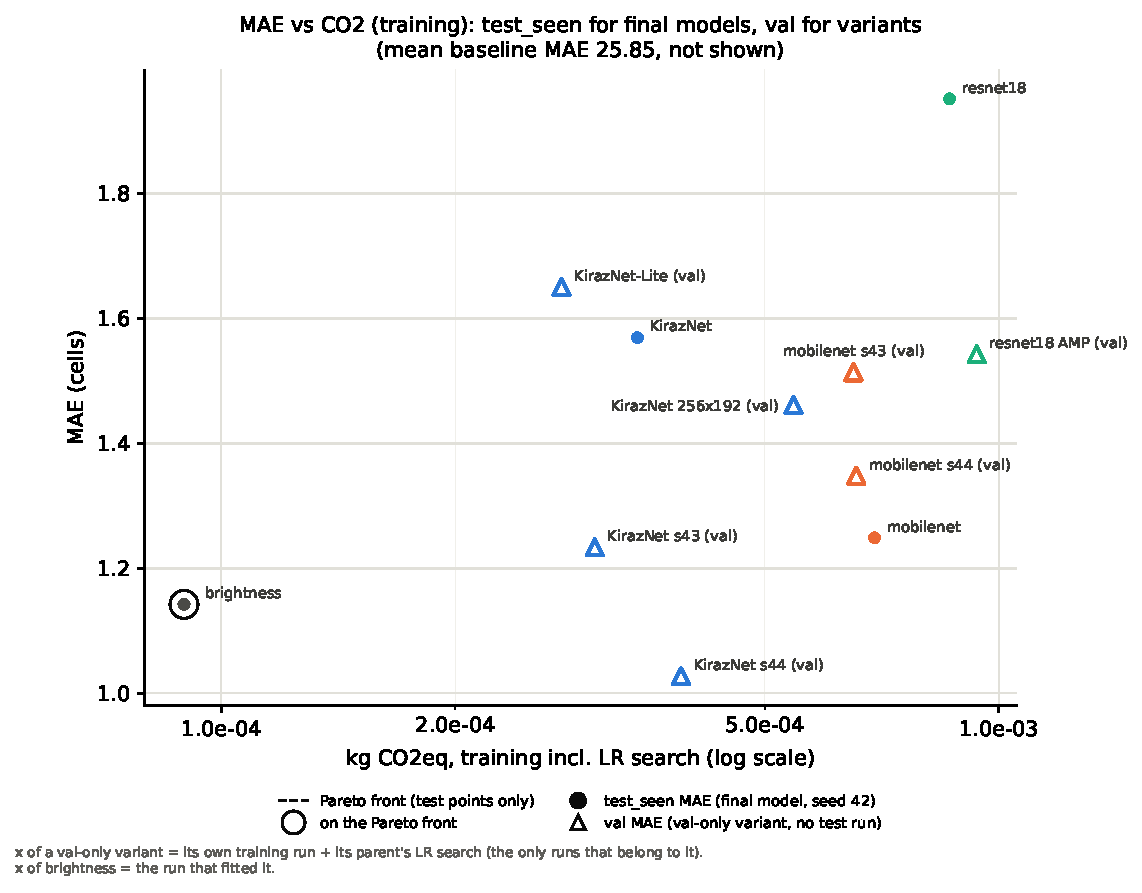
\includegraphics[width=0.82\linewidth]{mae_vs_co2_training.pdf}
\caption{MAE vs.\ training CO$_2$ incl.\ LR search (log $x$). Filled: test\_seen MAE of the final models;
open triangles: validation MAE of seeds and ablations (no test run). Circled: Pareto front of the plotted test
points. Linear $y$; the mean baseline (MAE 25.85) is not plotted.}
\label{fig:main}
\end{figure}

\textbf{Unseen counts.} On the four counts never seen in training, MAE stays in the same range
(brightness 1.15, \kn{} 1.37, MobileNetV3-Small 1.51, ResNet-18 2.13), and residuals at these counts
follow the neighbouring seen counts (Fig.~\ref{fig:resid}). The models therefore regress rather than
classify the 24 training levels.

\textbf{Blur and count.} Brightness, MobileNetV3-Small and ResNet-18 have flat error across blur levels;
\kn{}'s error grows from 1.43 (F1) to 1.78 (F48) (Fig.~\ref{fig:blur} in App.~B). By count
(Fig.~\ref{fig:resid}), \kn{} over-predicts by about one cell almost everywhere, while brightness and
MobileNetV3-Small under-predict the densest images (80+ cells), where overlapping nuclei no longer add
brightness linearly.

\begin{figure}[t]
\centering
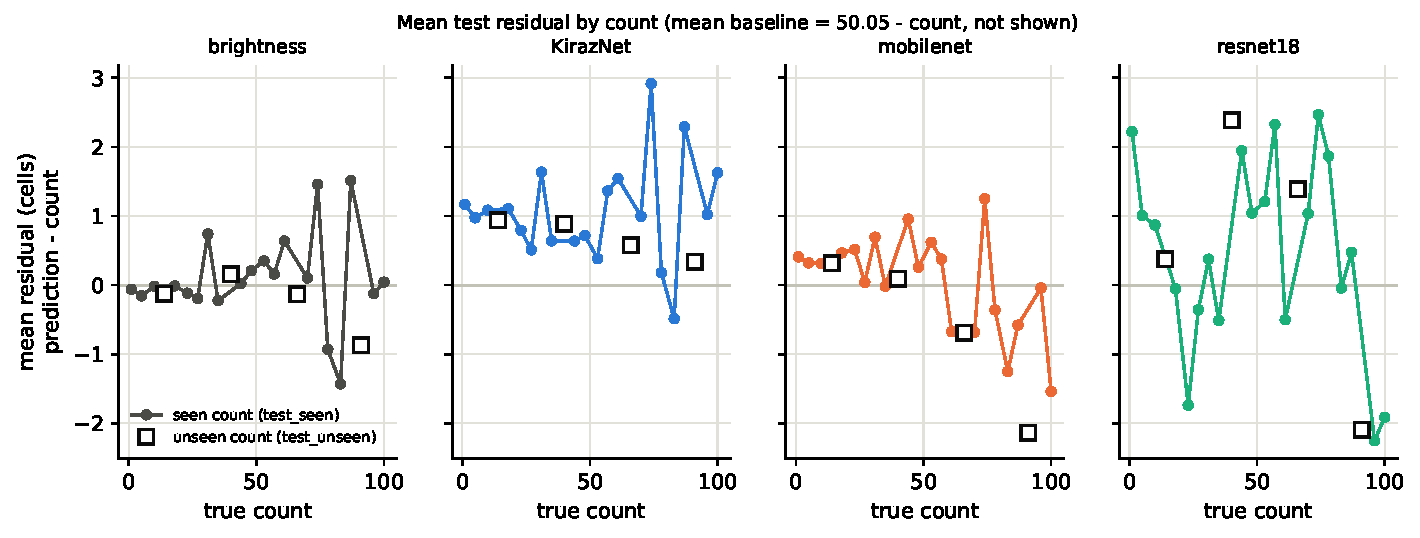
\includegraphics[width=\linewidth]{residual_by_count.pdf}
\caption{Mean test residual (prediction $-$ count) per true count; squares are the held-out counts.}
\label{fig:resid}
\end{figure}

% =====================================================================
\section{Ablations and efficiency techniques}

\begin{table}[h]
\centering\small
\caption{Validation results, seed 42 unless noted. Energy per step includes the periodic validation passes.
The \kn{} seed range on validation is 1.027--1.356 (0.33 cells).}
\label{tab:ablation}
\begin{tabular}{lrrrrr}
\toprule
Variant & Val MAE & Steps run & Energy (Wh) & mWh/step & MACs/img\\
\midrule
\kn{} $128\times96$ (reference) & 1.356 & 2{,}250 & 0.439 & 0.195 & 37.2\,M\\
\kn{} $256\times192$ & 1.462 & 1{,}500 & 0.873 & 0.582 & 148.6\,M\\
\kn{}-Lite (depthwise-separable) & 1.651 & 1{,}650 & 0.290 & 0.176 & 6.5\,M\\
ResNet-18 FP32 (final) & 2.047 & 1{,}800 & 1.095 & 0.608 & 424.9\,M\\
ResNet-18 mixed precision & 1.543 & 3{,}000 & 1.250 & 0.417 & 424.9\,M\\
ResNet-18 FP32, 600-step noise ref. & 1.762 & 600 & 0.364 & 0.606 & 424.9\,M\\
\bottomrule
\end{tabular}
\end{table}

\textbf{Resolution.} Four times the pixels cost $3.0\times$ the energy per step and did not improve
validation error (1.46 vs.\ 1.36, inside the seed range): $128\times96$ loses no useful information, as
the geometric check predicted.

\textbf{Depthwise-separable (\kn{}-Lite).} 7$\times$ fewer parameters (8{,}449) and 5.7$\times$ fewer MACs
saved only 10\% energy per step; error rose to 1.65 (just inside the seed range, so ``no clear
difference''). On this GPU, small depthwise layers are limited by memory traffic and kernel launches,
not arithmetic --- the same reason MobileNetV3-Small, with fewer MACs than \kn{}, is $7\times$ slower per
image on GPU (6.0 vs.\ 0.84\,ms). \emph{MACs are a poor proxy for energy; it has to be measured.}

\textbf{Mixed precision.} On ResNet-18, AMP cut energy per step by 31\% (0.417 vs.\ 0.608\,mWh) and time
per step by about 30\%. Two FP32 runs agree within 0.3\% (0.606 vs.\ 0.608), so the saving is far larger
than run-to-run noise.

\textbf{Early stopping.} Five runs stopped before 3{,}000 steps and skipped 5{,}850 steps in total, about
2.18\,Wh (1.0\,g CO$_2$eq), estimated as steps not run $\times$ each run's measured energy per step. It
saved most where it hurt most: ResNet-18 stopped at step 1{,}800 (Sec.~\ref{sec:why2}).

\textbf{Caching.} Decoding and resizing the 1{,}200 training TIFs took 11.5\,s and 0.128\,Wh; loading the
cache took 0.1\,s. Building the cache once cost 0.131\,Wh. Decoding in every one of the 61 epochs of the
final \kn{} run would have cost about 7.8\,Wh and 704\,s, 17 times the energy of that whole run (0.44\,Wh).
Both measurements are short runs below CodeCarbon's resolution, and the operating system would cache
some files, so the saving is an upper-end estimate --- but caching is by far the largest single saving.

% =====================================================================
\section{Why \kn{} failed the acceptance test}\label{sec:why}
These diagnostics are post-hoc and use validation data only; nothing was re-tuned and the test set was
not used again.
\begin{enumerate}\setlength\itemsep{1pt}
\item \textbf{A lucky checkpoint on a noisy curve.} With LR $3\cdot10^{-3}$, validation MAE jumps by up to an
order of magnitude between evaluations while the training loss is flat (Fig.~\ref{fig:curves}), most
likely because BatchNorm running statistics lag behind fast-changing weights in eval mode. The seed-42
checkpoint (1.356 at step 1{,}350) is $1.37\times$ better than the median of the last five evaluations
(1.857); for MobileNetV3-Small the ratio is only 1.05. Its validation score was therefore optimistic
(test 1.569), while MobileNetV3-Small, selected late in the low-LR phase, generalised (val 1.513, test 1.249).
\item \textbf{A systematic offset.} The seed-42 checkpoint over-predicts by +0.76 cells on validation
(16 of 20 counts); removing that offset would give 1.11 (optimistic, same data). It is the only \kn{}
seed with a positive offset; the same offset is visible on test (Fig.~\ref{fig:resid}).
\item \textbf{Seed variance.} \kn{} seeds reach 1.356, 1.234 and 1.027 on validation (seed 44 is below
brightness, 1.081). The pre-fixed seed 42 was the worst of the three. We kept it, as the protocol requires.
\end{enumerate}
The architecture is therefore able to reach brightness-level accuracy, but the selection procedure
(best of noisy evaluations at a high LR) is fragile. Selecting on a smoothed score (e.g.\ the median of
the last evaluations), a lower LR, or averaged weights (EMA) would likely be more robust; we did not test
these, to keep the protocol fixed.

\begin{figure}[t]
\centering
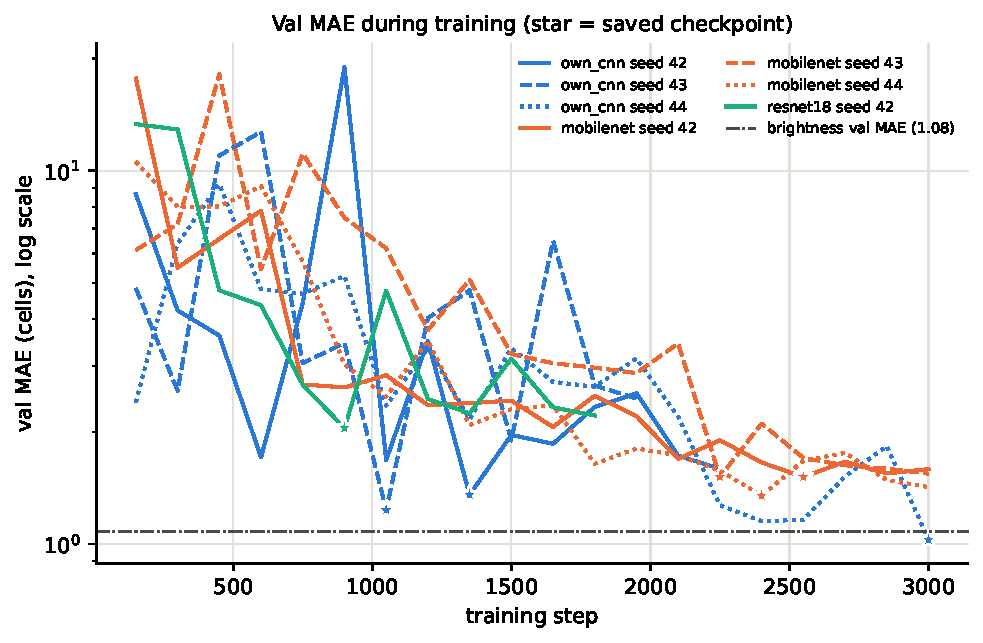
\includegraphics[width=0.85\linewidth]{val_curves.pdf}
\caption{Validation MAE during training (log $y$); stars mark the saved checkpoints; the dash-dot line is
the brightness baseline.}
\label{fig:curves}
\end{figure}

% =====================================================================
\section{Discussion and trade-offs}
\begin{itemize}\setlength\itemsep{1pt}
\item \textbf{The cheapest model is (almost) good enough.} A two-parameter linear model on mean brightness
is statistically tied with the best CNN and better than the others, with no training cost and orders of
magnitude less inference energy. For a green workflow, simple physical baselines should be tried before
deep models.
\item \textbf{Small is cheap but not automatically accurate.} \kn{} had the lowest training CO$_2$ among
CNNs and the fastest GPU inference, but pretrained MobileNetV3-Small was more accurate and more stable,
at 4$\times$ the CPU inference energy. Pretraining helps even on synthetic grey blobs, but its own
historical footprint is not in our numbers.
\item \textbf{Bigger is not better here.}\label{sec:why2} ResNet-18 was the most expensive and least accurate CNN: at
$128\times96$ its stride-heavy stem shrinks nuclei to about 1.5\,px, and early stopping ended its run at
step 1{,}800 (best at 900) before the low-LR phase; its mixed-precision twin, which ran 3{,}000 steps,
reached 1.54 on validation.
\item \textbf{Measure, do not estimate.} MACs predicted neither GPU time nor energy (depthwise layers,
MobileNet).
\end{itemize}

\section{Limitations}
\begin{itemize}\setlength\itemsep{1pt}
\item Synthetic data only; brightness works because illumination is stable, which real microscopy does not
guarantee. Cells cut by the image border can make the visible count lower than the label.
\item One test set of 100 scenes; one final seed per model (by design); ResNet-18 has no seed spread; three
CNN-vs-brightness comparisons without multiple-comparison correction.
\item LR chosen from 300-step trials (favours fast starters); early stopping on a noisy validation curve
cut ResNet-18 short.
\item Energy: CPU and GPU measured, RAM modelled; runs under 15\,s below resolution; laptop thermal state
not logged. AI-assistant usage, data download and ImageNet pre-training are not counted.
\item Two rule revisions were made after a check had run (disclosed, App.~A); the brightness comparison was
added after seeing its validation score.
\end{itemize}

\section{Conclusion}
We built a fully measured, leakage-free pipeline for counting cells in BBBC005 at a total cost of
15.1\,g CO$_2$eq. Our small CNN, \kn{}, was the cheapest CNN to train but missed the acceptance threshold
by 0.13 cells, because the pre-fixed checkpoint was selected on a noisy validation curve and carries a
systematic offset. The more important finding is that a two-parameter brightness model matches or beats
every CNN at a tiny fraction of the energy. The greenest model is the one that does not need a GPU.

\paragraph{AI tools.} Claude, ChatGPT and Gemini were used for planning, rule drafting, code and writing;
see the separate AI Usage Report. All numbers in this report are generated by scripts from logged runs
(\texttt{results/summary.md}).

% =====================================================================
\begin{thebibliography}{99}\small
\bibitem{ljosa2012} V.~Ljosa, K.~L.~Sokolnicki, A.~E.~Carpenter. Annotated high-throughput microscopy image
sets for validation. \emph{Nature Methods} 9:637, 2012.
\bibitem{lehmussola2007} A.~Lehmussola, P.~Ruusuvuori, J.~Selinummi, H.~Huttunen, O.~Yli-Harja. Computational
framework for simulating fluorescence microscope images with cell populations. \emph{IEEE TMI} 26(7), 2007.
\bibitem{zhao2024} P.~Zhao, L.~Hong, Y.~Wang. Abnormal gait recognition with millimetre-wave radar based on
perceptual loss and convolutional temporal autoencoder. \emph{IET Radar, Sonar \& Navigation} 18(12):2630--2641, 2024. doi:10.1049/rsn2.12664.
\bibitem{lempitsky2010} V.~Lempitsky, A.~Zisserman. Learning to count objects in images. \emph{NeurIPS}, 2010.
\bibitem{xie2018} W.~Xie, J.~A.~Noble, A.~Zisserman. Microscopy cell counting and detection with fully
convolutional regression networks. \emph{Computer Methods in Biomechanics and Biomedical Engineering:
Imaging \& Visualization}, 2018.
\bibitem{strubell2019} E.~Strubell, A.~Ganesh, A.~McCallum. Energy and policy considerations for deep learning
in NLP. \emph{ACL}, 2019.
\bibitem{schwartz2020} R.~Schwartz, J.~Dodge, N.~A.~Smith, O.~Etzioni. Green AI. \emph{Communications of the
ACM} 63(12), 2020.
\bibitem{lacoste2019} A.~Lacoste, A.~Luccioni, V.~Schmidt, T.~Dandres. Quantifying the carbon emissions of
machine learning. arXiv:1910.09700, 2019.
\bibitem{codecarbon} CodeCarbon contributors. CodeCarbon: track the emissions of your compute (software), version 3.3.2. \url{https://github.com/mlco2/codecarbon}.
\bibitem{he2016} K.~He, X.~Zhang, S.~Ren, J.~Sun. Deep residual learning for image recognition. \emph{CVPR}, 2016.
\bibitem{howard2019} A.~Howard et al. Searching for MobileNetV3. \emph{ICCV}, 2019.
\bibitem{goodfellow2016} I.~Goodfellow, Y.~Bengio, A.~Courville. \emph{Deep Learning}. MIT Press, 2016.
\end{thebibliography}

% =====================================================================
\appendix
\section{Pre-registered rules and their revisions}
All rules are in \texttt{docs/decision\_rules.md} (machine-readable copy \texttt{configs/rules.json}); every
stage was tagged in git before the next one used it.
\begin{center}\footnotesize
\begin{tabular}{p{0.25\linewidth}p{0.5\linewidth}p{0.17\linewidth}}
\toprule
Tag & Frozen content & Before \\
\midrule
\texttt{rules-v1} & split, stain/resolution/blur rules, baselines, acceptance, test protocol & any check or split\\
\texttt{split-v1} & scene split (seed 42), held-out counts & any image was viewed\\
\texttt{rules-v1.1}, \texttt{data-v2} & revised resolution check; stain w1, $128\times96$, F1/F26/F39/F48 & caching\\
\texttt{cache-v1} & cached arrays, normalisation, baselines on val & any model\\
\texttt{rules-v2} & architecture, training, early stopping, LR search, seeds, measurement & any training\\
\texttt{rules-v2.1} & zero-initialised output layer for all models & LR search\\
\texttt{search-v1}, \texttt{train-v1}, \texttt{ablation-v1} & LR choices, final models, ablations & test\\
\texttt{test-v1} & single test run per final model, results & analysis\\
\bottomrule
\end{tabular}
\end{center}
\textbf{Revision 1 (rules-v1.1).} The first resolution check found peaks with a 1\,px smoothing, far below the
nucleus size (31.7\,px at native resolution), so it counted texture \emph{inside} nuclei (154--185 peaks in
images with 100 nuclei) and rejected every resolution, falling back to $348\times260$ ($7.4\times$ the pixels of
$128\times96$). We changed one principle --- measure peaks at nucleus scale ($\sigma=d/4$) --- and kept every
threshold; the revised check found 86--93 peaks and passed $128\times96$. The revision was made after seeing the
first outcome, so it is not pre-registered; both outcomes are kept in the repository.

\textbf{Revision 2 (rules-v2.1).} Zero-initialised output weights for all models, decided after a 20-step smoke
test and before any LR search or training (Sec.~3).

\textbf{Visual checks.} Stain (Fig.~\ref{fig:stain}): w1 = nuclei, contrary to the documentation. Resolution:
nucleus diameter 5.8\,px at $128\times96$ ($\geq3$\,px required); 99.3\% of resolvable neighbour pairs stay
resolved ($\geq90\%$ required). Blur: a high-pass similarity measure selected F1, F26, F39, F48 (four levels, the
minimum allowed by the image-count requirement).

\begin{figure}[h]
\centering
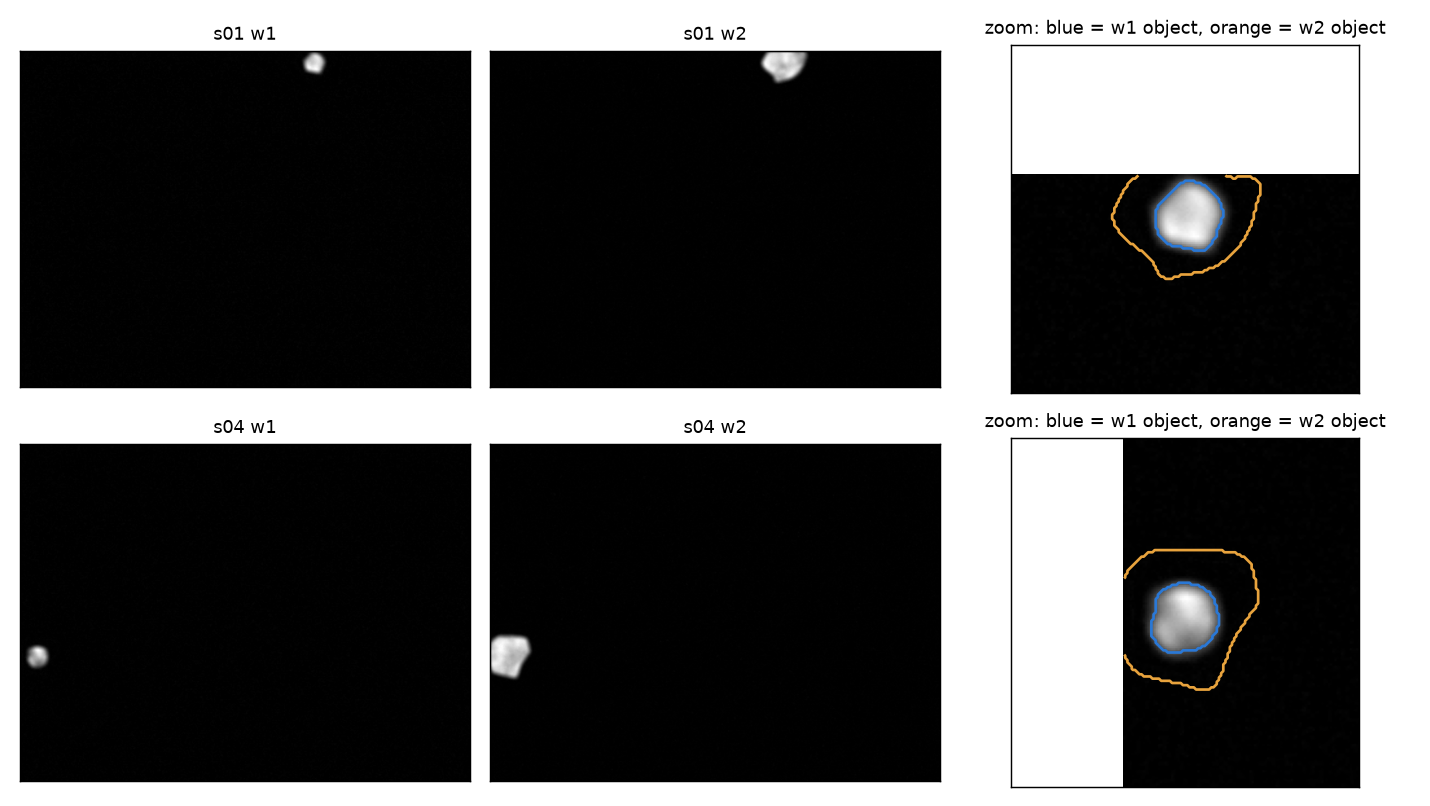
\includegraphics[width=0.9\linewidth]{stain_overlay.png}
\caption{Stain check on C1 F1 (training samples 1 and 4): the w1 object (blue) lies inside the w2 object
(orange) and is 3--4$\times$ smaller, so w1 is the nuclei stain, contrary to the documentation.}
\label{fig:stain}
\end{figure}

\section{Additional figures}
\begin{figure}[h]
\centering
\begin{subfigure}{0.49\linewidth}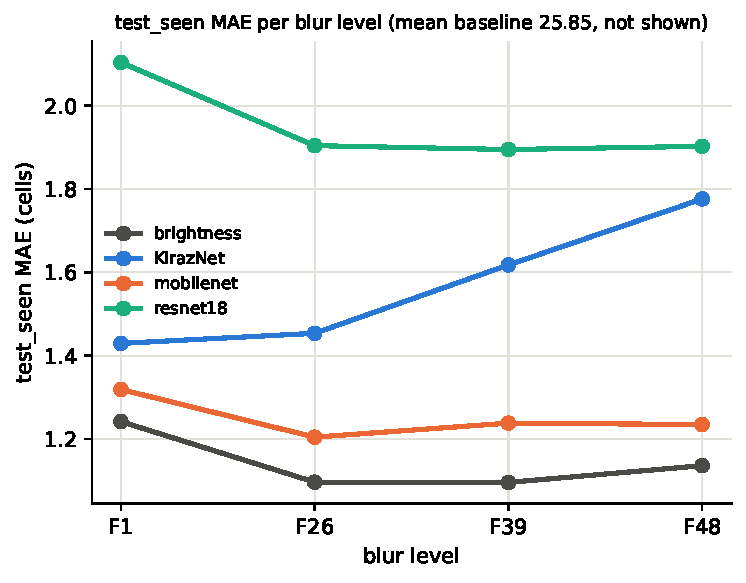
\includegraphics[width=\linewidth]{test_mae_by_blur.pdf}
\caption{Test MAE per blur level.}\label{fig:blur}\end{subfigure}
\begin{subfigure}{0.49\linewidth}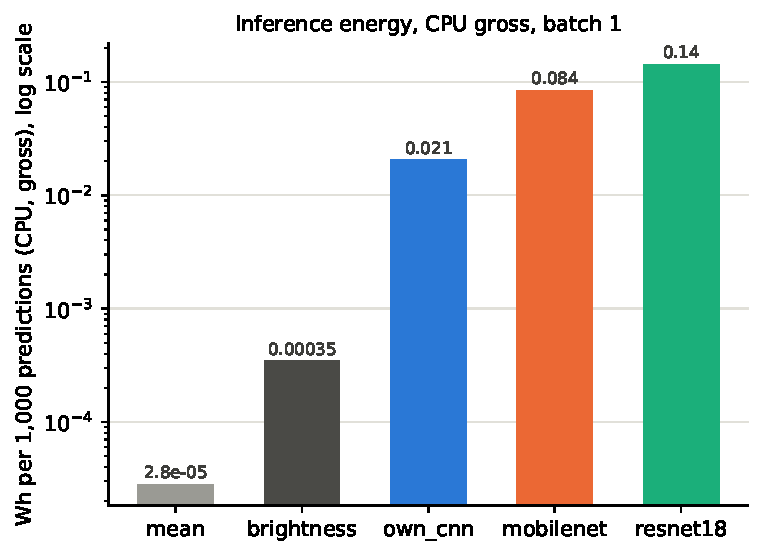
\includegraphics[width=\linewidth]{energy_per_1000.pdf}
\caption{CPU energy per 1{,}000 predictions (log).}\end{subfigure}
\caption{Error by blur level and inference energy.}
\end{figure}

\section{Reproducibility}
The repository contains all code (\texttt{src/}, \texttt{scripts/}), the frozen rules, the split file with its
SHA-256, every run folder with its \texttt{emissions.csv}, \texttt{config.json} and \texttt{metrics.json}
(\texttt{runs/index.csv} lists all runs, including failed ones), all results and figures, and the \kn{}
seed-42 weights (0.25\,MB). \texttt{README.md} lists the exact commands to rebuild the cache, train every model,
run the single test evaluation, and regenerate every table and figure; \texttt{results/summary.md} maps every
number in this report to the file it comes from. Seeds are fixed and cuDNN is deterministic; two repeated runs
gave bit-identical weights.

\begin{figure}[h]
\centering
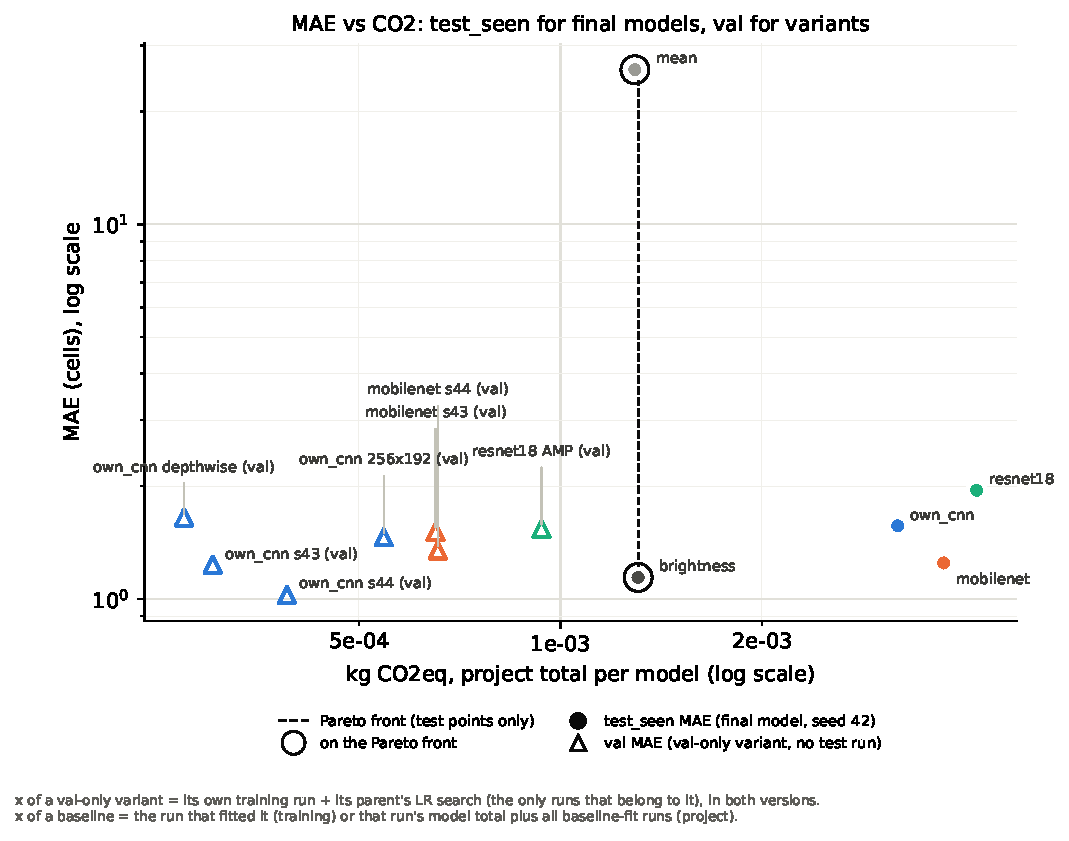
\includegraphics[width=0.75\linewidth]{mae_vs_co2_project.pdf}
\caption{MAE vs.\ project CO$_2$ per model (all runs named after the model), test points only.}
\label{fig:project}
\end{figure}

\end{document}
